\chapter{The Large Hadron Collider}
\label{ch:lhc}
\begin{chapquote}{Pablo Picasso}
{Every act of creation begins with an act of destruction.}
\end{chapquote}


The LHC is a 27~km circumference particle accelerator straddling the border between France and Switzerland \cite{LHC}. It now collides bunches of $10^9$ protons every 25~ns at a center of mass energy of 13~TeV \cite{ATLAS_long}.
Bunches of protons are used since the proton radius is about 1~fm, and thus the probability of a head-on collision between single protons is increased by increasing the number of colliding particles.  We expect about 20 collisions per given bunch crossing at the LHC \cite{PU}.

Since the proton is not an elementary particle, but rather a baryonic resonant QCD bound state, even a head-on collision will not have all of the available energy concentrated at a point.
The proton is a composite particle made up of two up and one down valence quarks, along with a sea of virtual quarks and gluons that spontaneously come out of the vacuum because of the uncertainty relation $\Delta x \Delta p \geq \hbar / 2$.  
The 6.5~TeV per proton is distributed among these partons\footnote[3]{A parton is a constituent of a hadron.}.  Therefore, to look at the high-energy regime, we are interested in a ``hard scatter'' where a single quark or gluon carrying a large fraction of one proton's momentum collides with a high energy constituent of the other proton, lending to the production of one or more Higgs bosons.

\begin{itemize}
	\item History
	\item Collider Stats
	\item I should make a set of slides (or app) making sure that I know what the dipole and focusing magnets do!!
\end{itemize}

\begin{figure}[hbt]
\centering
\subfloat[]{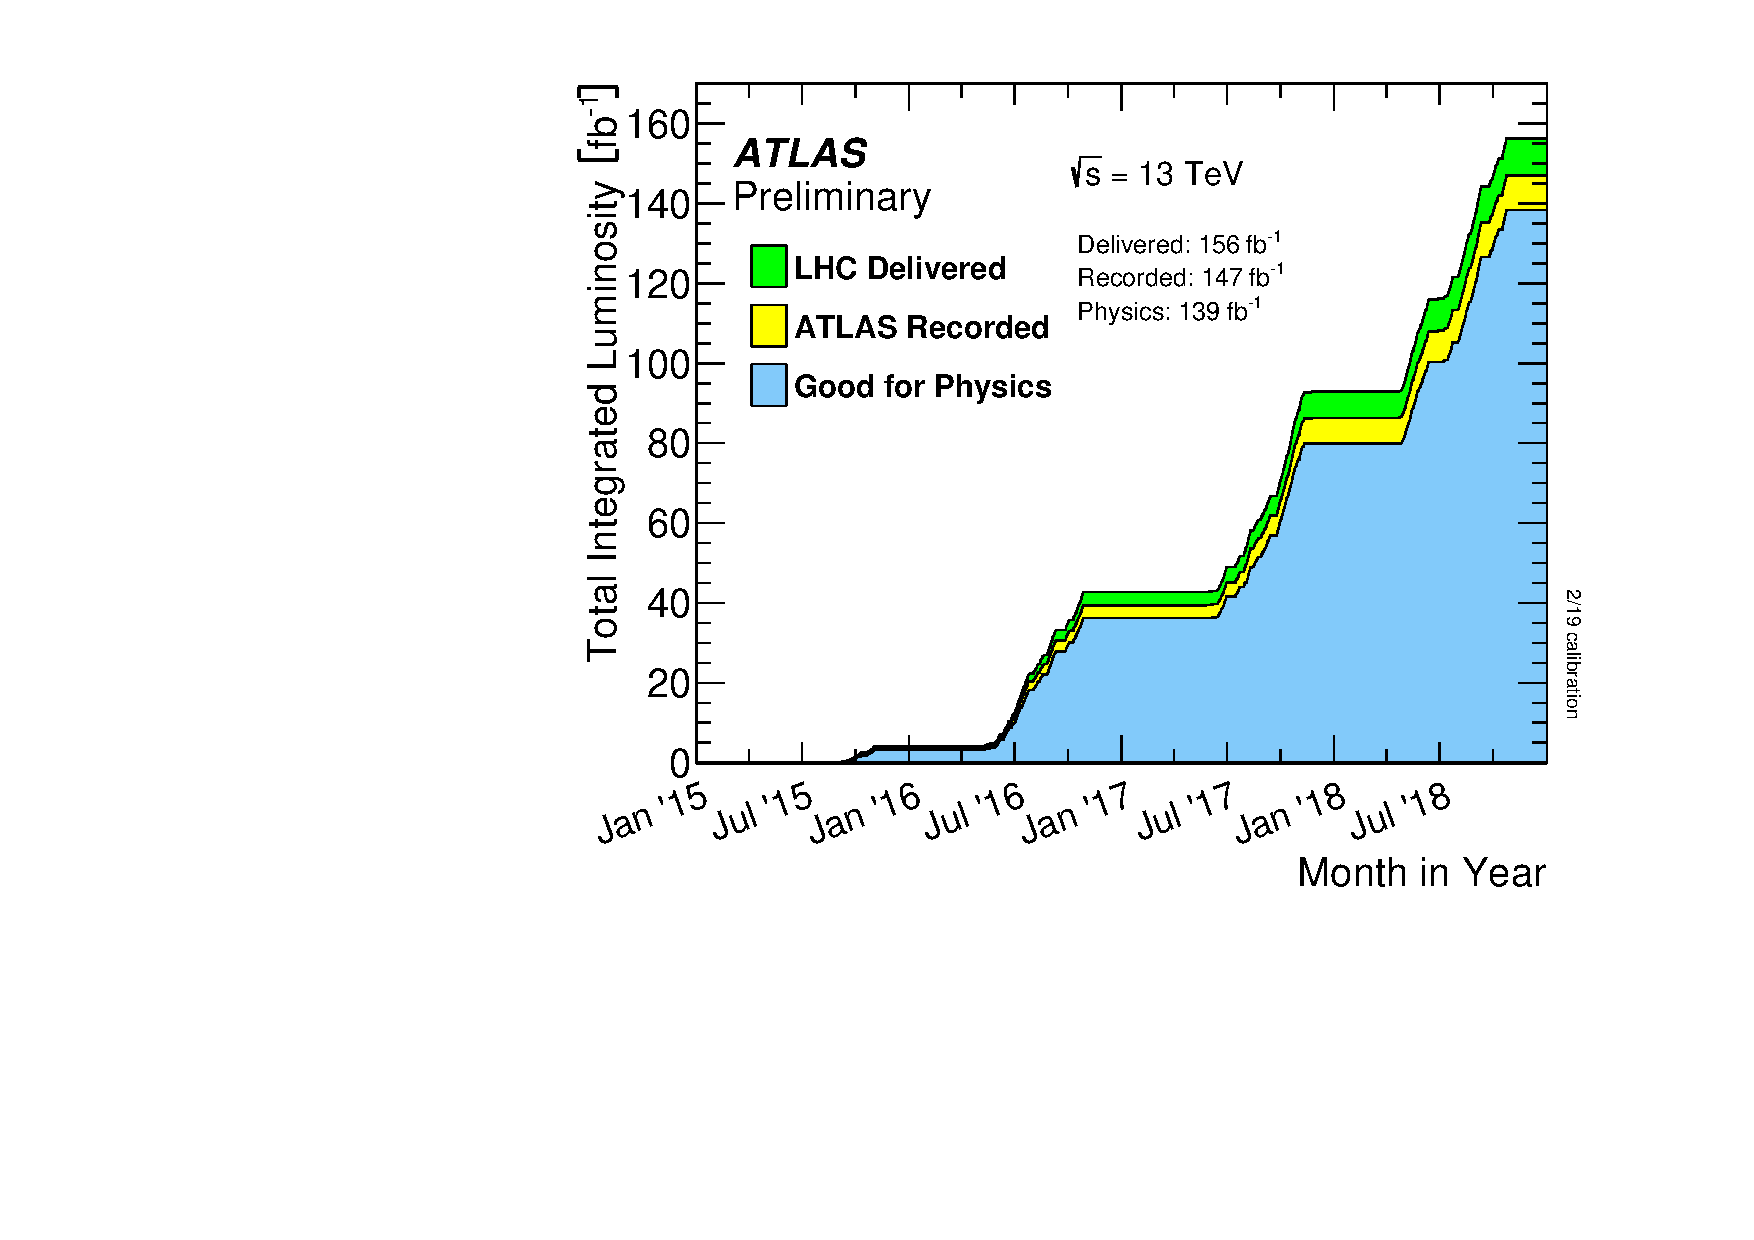
\includegraphics[width=.45\textwidth]{{figures/lhc/intlumivstimeRun2DQall.pdf}}}
\subfloat[]{
	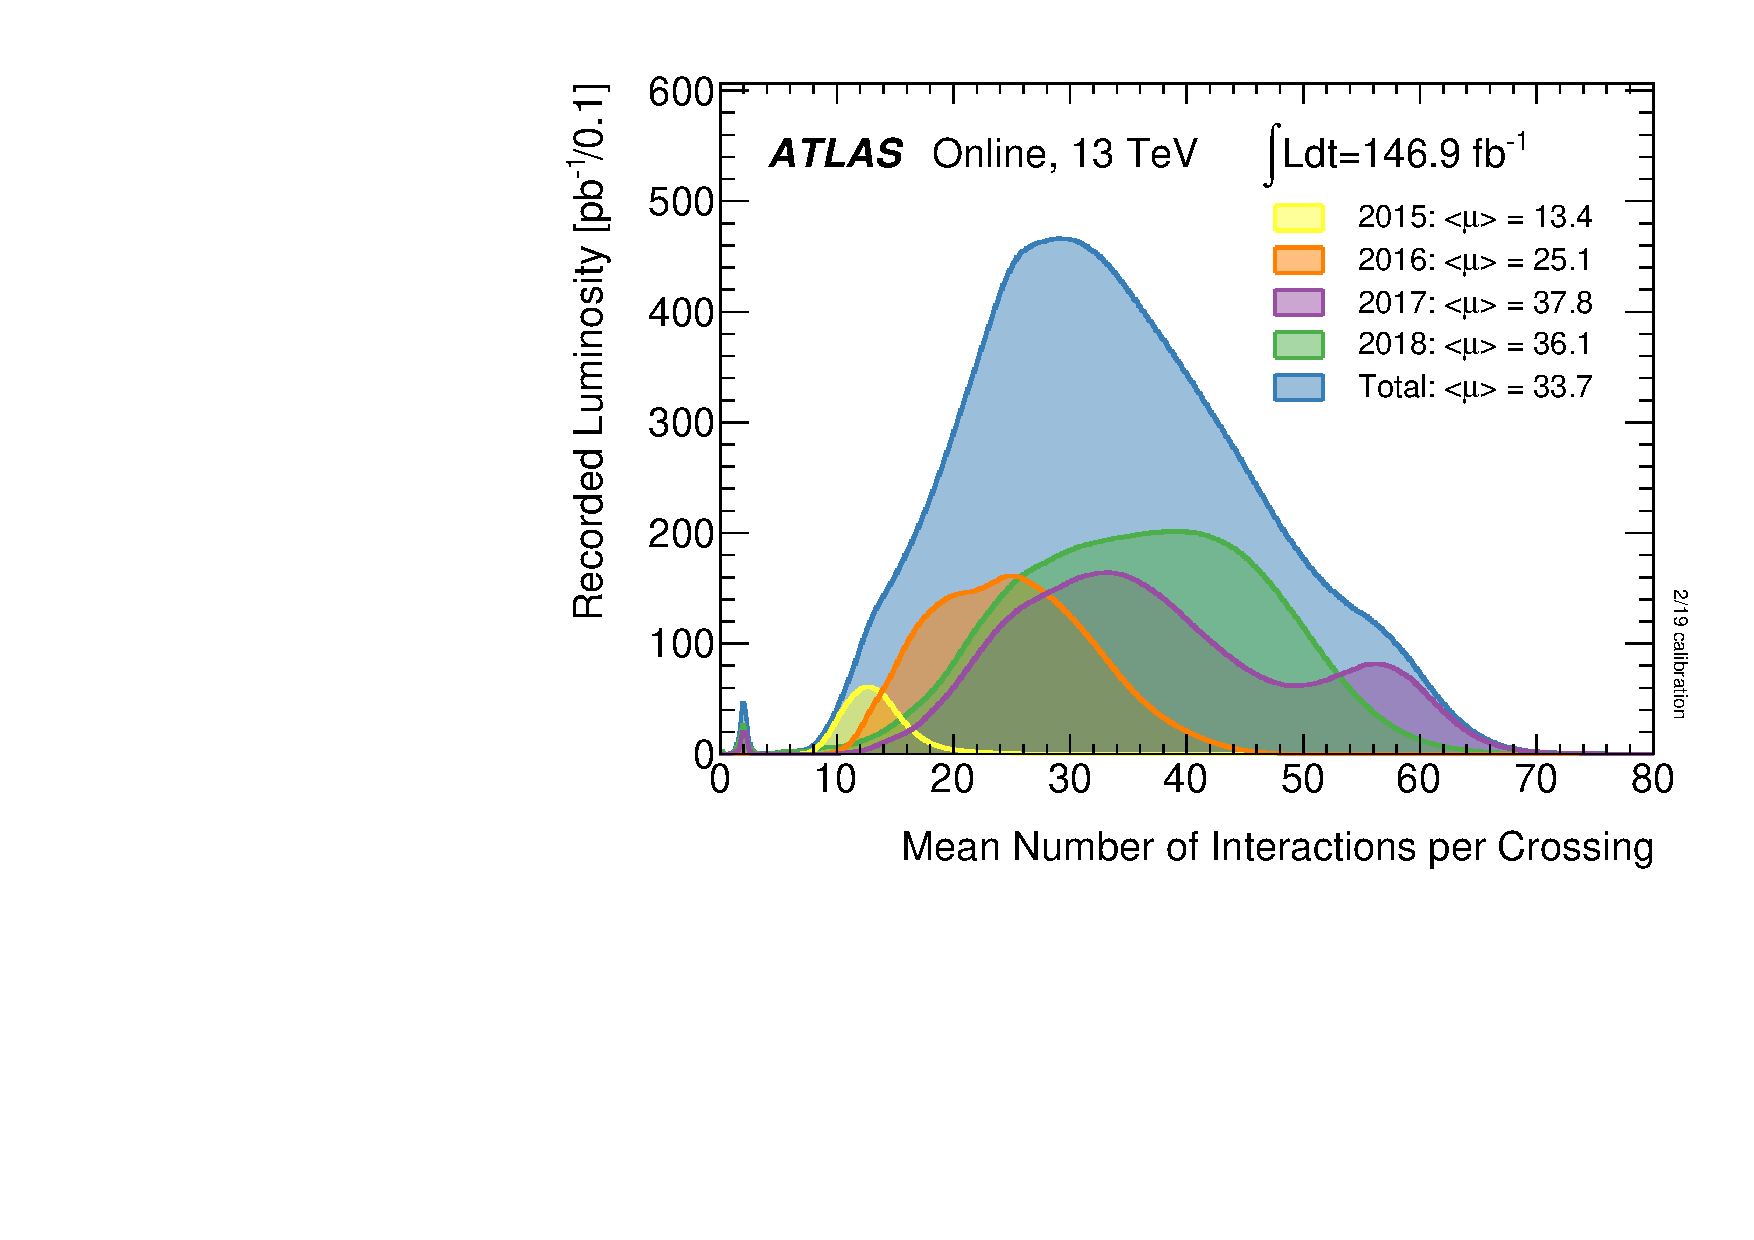
\includegraphics[width=.45\textwidth]{{figures/lhc/mu_2015_2018.pdf}}
	\label{PU density profile for Run~2 data taking.}
	}
\caption{Need to cite: https://twiki.cern.ch/twiki/bin/view/AtlasPublic/LuminosityPublicResultsRun2\#Pileup\_Interactions\_and\_Data\_Tak}
\end{figure}